% !TEX root = main.tex
%
% Introduction
%
Parsing %variant of membership problem for formal languages
%- given a language model and an input word $s$, compute a derivation of the model that yields $s$.
is the problem %process 
of structuring a linear representation in input %typically
(a finite word over an alphabet) according to a language model. % (a formal grammar).
% natural language, programming language, 
%
Most of the context-free parsing approaches~\cite{GruneJacobs08parsing}  
assume a finite and reasonably small input alphabet. %models and algorithms 
Such a restriction makes perfectly sense in the context of NLP tasks 
like constituency parsing or of programming languages compilers or interpreters.
Considering large or infinite alphabets can however be of practical interest
in other cases.
%
For instance, when dealing with large characters encodings such as UTF-16, % processing strings in 
\eg for vulnerability detection in Web-applications~\cite{dAntoni21CACM}, 
%
for the analyse (\eg validation or filtering) 
of data streams or serialization of structured documents 
(which may contain textual or numerical attributes)~\cite{Segoufin06csl}, 
or for processing timed execution traces~\cite{Bouyer03algebraic}.
% algebraic definition of a class of data languages 
% (notion of monoid recognizability, based on registers, comparable to Bojancszik et al. data words)
Regarding the latter case, we describe %briefly 
at the end of the paper 
a parse-based approach to automated music transcription,
where a symbolic music performance, 
presented as a sequence of timed musical events, % timestamped
% a symbolic representation of a music performance 
is converted into a structured score in Common Western Music Notation~\cite{foscarin:hal-01988990}.
%generalizes weighted parsing: 
%finding the best derivation for a weighted grammar. 

Various extensions of language models for handling infinite alphabets have been studied.
%words carrying data values in an infinite domain (e.g. integers) e.g. data processing 
For instance, some automata with memory extensions 
allow restricted storage and comparison of input symbols, 
%and correspond with logics, 
(see~\cite{Segoufin06csl} for a survey),
with pebbles for marking positions~\cite{NevenSchwentickVianu04FSMinfinite}, 
registers~\cite{KaminskiFrancez94}, 
or %computations in 2 steps
the possibility to compute on subsequences 
with the same attribute values~\cite{Bojanczyk11FO2}. % data words automata.
%
%for the and verification of infinite state systems 
%(model checkers: alphabet = long bit-vectors)
%...For the representation of  in model checking, verification and 
The automata at the core of model checkers
compute on input symbols represented by large bitvectors~\cite{Vardi07ciaa} %\cite{BaierKatoen08MC}
(sets of assignments of Boolean variables) %propositional variables)
and in practice,  %implementation
each transition accepts a set of such symbols (instead of an individual symbol), 
represented by Boolean formula or Binary Decision Diagrams.
%
Following a similar idea, % and generalizing,
in symbolic automata (\SA)~\cite{dAntoniVeanes17CAV,dAntoni21CACM}, 
the transitions are guarded by predicates over infinite alphabet domains.
With closure conditions on the sets of such predicates, % (alphabet theories), 
all the good properties enjoyed by automata over finite alphabets are preserved.

Other extensions of language models  %(automata and grammars) 
help in dealing with non-determinism, by the computation of weight values. 
With an ambiguous grammar, there may exists several derivations 
(\emph{abstract syntax trees} -- AST), % \ie the result of an analyze.
yielding one input word. % structuring a word, 
The association of one weight value %in semiring domain
to each derivation permits to select a best one (or $n$ bests). % a fixed number of bests 
% = ...a ranking of derivations 
This is roughly the principle of \emph{weighted parsing}
approaches~\cite{Goodman99SemiringParsing,Nederhof03weightedParsing,MorbitzVogler19weighted-parsing}.
In \emph{weighted language models}, 
like \eg probabilistic context-free grammars % (CFG),
and weighted automata (\WA) \cite{Droste09handbook},
a weight value is associated to each transition rule, % production rule
and the rule's weights can be combined with a associative product operator~$\otimes$ into 
the weight of a derivation.
A second operator~$\oplus$, associative and commutative, 
is moreover used to handle ambiguity of the model, 
by summing the weights of the possibly several (in general exponentially many) AST %syntax trees 
associated to a given input word.
Typically, $\oplus$ will select the best of two weight values.
%Intuitively,~$\oplus$ selects, or ranking, the syntax trees.
The weight domain, equipped with these two operators is assumed, at minima, 
to form a \emph{semiring} %$\Semiring$ 
where $\oplus$ can be extended to infinite sums, 
%\cite{Eilenberg74automata}
such as the Viterbi semiring and the tropical min-plus algebra, see Figure~\ref{fig:semirings}. 
%of domain $\mathbb{R}^+ \cup \{ +\infty\}$, 
%where $\oplus$ is min and $\otimes$ is plus .
%by ranking 
%making the weight domain a semiring.
%Some efficient specialized parsing algorithms~\cite{Huang05kbest} have been proposed in this context 
%% models represented as hypergraphs \cite{Huang05kbest}
%in order to compute the $n$ best syntax trees of a given input word without having to enumerate them all.
%Generally based on dynamic programming, these algorithms rely on 
%additional algebraic properties of~$\Semiring$.
%-- see \eg~\cite{Huang05kbest} for some NLP applications.
%The extraction of $n$ best list is useful 
%the problem: quantitative parsing or symbolic parsing
%of parsing of words over infinite input alphabet.

In this paper, we present a uniform framework for weighted parsing over infinite input alphabets.
It is based on weighted %finite states 
language models generalizing 
both~\SA, with functions in an arbitrary semiring instead of Boolean guards, 
and~\WA, by handling infinite alphabets -- Figure~\ref{fig:hierarchy}.
%***
%some weighted language models
%model of weighted CFG 
%computing on words over infinite input alphabets %sets of terminal symbol
%- but with finite sets of states and transitions rules. 
% non-terminals and production rules).
In their transition rules, input symbols appear as variables %(parameters)
and the weight associated to a transition rule is a function of these variables.
%
\begin{figure}
\centering
\begin{tikzpicture}
\node (NFA) at (0,4) {%
  \(
  \begin{array}{c} 
  \mathsf{NFA} : \Sigma_{\mathsf{fin}}^* \to \mathbb{B}\\
  q \xrightarrow{a} q' \quad  a \in \Sigma_\mathsf{fin}
  \end{array} 
  \)
};
%
\node (WA) at (-2,2) {%
  \(
  \begin{array}{c} 
  \mathsf{WA} : \Sigma_{\mathsf{fin}}^* \to \mathbb{S}\\
  q \xrightarrow{a, w} q' \quad  a \in \Sigma_\mathsf{fin}, w \in \mathbb{S}
  \end{array} 
  \)
};
%
\node (SA) at (2,2) {%
  \(
  \begin{array}{c} 
  \mathsf{SA} : \Sigma_{\mathsf{inf}}^* \to \mathbb{B}\\
  q \xrightarrow{\phi} q' \quad \phi : \Sigma_\mathsf{inf} \to \mathbb{B}
  \end{array} 
  \)
};
%
\node (SWA) at (0,0) {%
  \(
  \begin{array}{c} 
  \mathsf{SWA} : \Sigma_{\mathsf{inf}}^* \to \mathbb{S}\\
  q \xrightarrow{\phi} q' \quad \phi : \Sigma_\mathsf{inf} \to \mathbb{S}
  \end{array} 
  \)
};
\draw[->] (NFA)--(WA);
\draw[->] (NFA)--(SA);
\draw[->] (WA)--(SWA);
\draw[->] (SA)--(SWA);
%\begin{array}{c} \mathsf{NFA} : \Sigma^* \to \mathbb{B} \end{array} 
\end{tikzpicture}
\caption{Classes of Symbolic/Weighted Automata. 
$\Sigma_\mathsf{fin}$ is a finite alphabet, 
$\Sigma_\mathsf{inf}$ is a countable alphabet,
$\mathbb{B}$ is the Boolean algebra, 
$\mathbb{S}$ is an arbitrary commutative semiring, 
$q \xrightarrow{\dots} q'$ represents the form of a transition between states $q$ and $q'$.}
\label{fig:hierarchy}  
\end{figure}
%
%This approach is close to the case of 
%Symbolic Automata (SA)~\cite{dAntoniVeanes17CAV,dAntoni21CACM}, 
%except that the domain for weight values is not restricted to be Boolean, 
%like for the guards in the rules of SA, 
%but can be an arbitrary commutative semiring (assuming some restrictions).
%
The models presented here are finite automata called symbolic-weighted (\SWA),
transducers (\SWT) and pushdown automata,
with a visibly restriction~\cite{AlurMadhusudan09nested} (\SWVPA).
%\wrt an edit distance
The latter model of automata computes on \emph{nested words}~\cite{AlurMadhusudan09nested}, 
a structured form of words parenthesized with markup symbols, 
corresponding to a linearization of trees.
In the context of parsing, they are used here to represent (weighted) AST of CF grammars.
More precisely, a \SWVPA $A$ associates a weight value $A(t)$ % \in \Semiring$ 
to a given a nested word $t$, which is the linearization of an AST. %representing a parse tree.
%
On the other hand, 
a \SWT is used to define a distance $T(s, t)$ between two finite words $s$ and $t$
over an infinite alphabet, following~\cite{Mohri03EDWA}.
Then, the \emph{SW-parsing} problem aims at %computing 
finding $t$ minimizing 
$T(s, t) \otimes A(t)$ (\wrt the ranking defined by $\oplus$)
-- this value is called the distance between $s$ and $A$ in~\cite{Mohri03EDWA}.
%
Similarly to weighted-parsing 
methods~\cite{Goodman99SemiringParsing,Nederhof03weightedParsing,MorbitzVogler19weighted-parsing}, 
our approach proceeds in two steps, 
based on properties of the SW models. 
The first step is a Bar-Hillel construction where, 
given a \SWT $T$, a \SWVPA $A$, and an input word $s$, 
a \SWVPA $A_{T, s}$ is built, such that for all $t$, $A_{T, s}(t) = T(s, t) \otimes A(t)$.
In the second step, a best AST $t$ is found by applying to $A_{T, s}$ 
a best search algorithm similar to shortest distance in graphs~\cite{Mohri02semiring,Huang05kbest}.
%In expressiveness, they are equivalent to weighted CFG. 
%and can be used in a general approach for parsing over infinite input alphabets.
%
%Let $A$ be a \SWVPA, associating $A(w) \in \Semiring$ 
%to a given a nested word $w$ (representing a parse tree),
%and let a \SWT compute a distance $d$, in $\Semiring$, 
%between 2 strings over respectively an infinite input alphabet and the 
%same (infinite) alphabet of $A$.
%Then, the problem of Symbolic Weighted Parsing is, 
%given an input string $s$, to find a nested word $w$ minimizing 
%(according to the ranking defined by $\oplus$)
%the distance $d(s, w) \otimes A(w)$ between $s$ and $A$, 
%as defined in~\cite{Mohri03EDWA}.

% First one general edit-distance is defined by a weighted word 
% transducer~\cite{Mohri}
% %Symbolic automata transducers are extended models~\cite{VeanesdAntoniJACM}
% %dealing with infinite set of input symbols...
% value in a semiring...

The main contributions of the paper are: 
($i$)~the introduction of automata, \SWA, transducers, \SWT (Section~\ref{section:SWA}),
and visibly pushdown automata \SWVPA (Section~\ref{sec:SWVPA}),
generalizing the corresponding classes of symbolic and weighted models, 
%for the weighted computation on (nested) words over infinite alphabets;  
($ii$)~a polynomial best-search algorithm for \SWVPA, %(Section~\ref{sec:best})
% a framework for parsing over infinite alphabets, 
and ($iii$)~a uniform framework (Section~\ref{sec:parsing}) for parsing over infinite alphabets, 
the keys to which are 
($iii.a$)~the \SWT-based definition of generic edit distances between input and output words,
and ($iii.b$)~the use of nested words, and \SWVPA, 
instead of syntax trees and grammars. %(\S~\ref{sec:trees}).
%
Finally, Section~\ref{sec:transcription} describes
the implemented application %of this approach 
to automated music transcription
that motivated this study.

%based these models and on generic def. of distances;
%the use of VPA for parsing, word instead of trees, use comparison input-output.
%and best-search

%In Section~\ref{section:SWA} we introduce \SWA and \SWT.
%Then \SWVPA are defined in Section~\ref{sec:SWVPA}, 
%where a polynomial 1-best algorithm is described that can be use to solve
%Symbolic Weighted Parsing, as described Section~\ref{sec:parsing}.
%Finally, in Section~\ref{sec:transcription}, we present an application 
%of this approach to automated music transcription that has been implemented.
